\chapter{Arhitektura i dizajn sustava}
		
		Na arhitekturu sustava najveći utjecaj imali su principi oblikovanja: Podijeli pa vladaj, Zadrži razinu apstrakcije te Oblikuj za prenosivost. Princip Podijeli pa vladaj očituje se u podijeli sustava na manje komponente radi povećane razumljivosti te lakše zamjene dijelova i ponovnog korištenja. Princip Zadrži razinu apstrakcije omogućava razumijevanje poante podsustava bez poznavanja nepotrebnih detalja. Korištenje Jave kao objektno orijentiranog programskog jezika omogućuje nam upotrebu razreda, podatkovnih apstrakcija koje sadrže proceduralne apstrakcije (metode). Osim upotrebe razreda Java omogućuje rad na više platformi, čime je osigurana prenosivost.
		
	Organizacija sustava s najviše razine apstrakcije je klijent-poslužitelj-baza podataka. Klijenta predstavlja preglednik weba koji omogućuje korisniku slanje zahtjeva poslužitelju protokolom HTTP \textit{(engl. Hyper Text Transfer Protocol)}. Poslužitelj je server koji poslužuje te zahtjeve, prosljeđuje ih web aplikaciji koja se pokreće preko poslužitelja te vraća odgovore koji se prikazuju preko klijenta (preglednika). Podaci su spremljeni u bazi podataka te joj po potrebi pristupa web aplikacija koristeći SQL upite.
					\begin{figure}[H]
						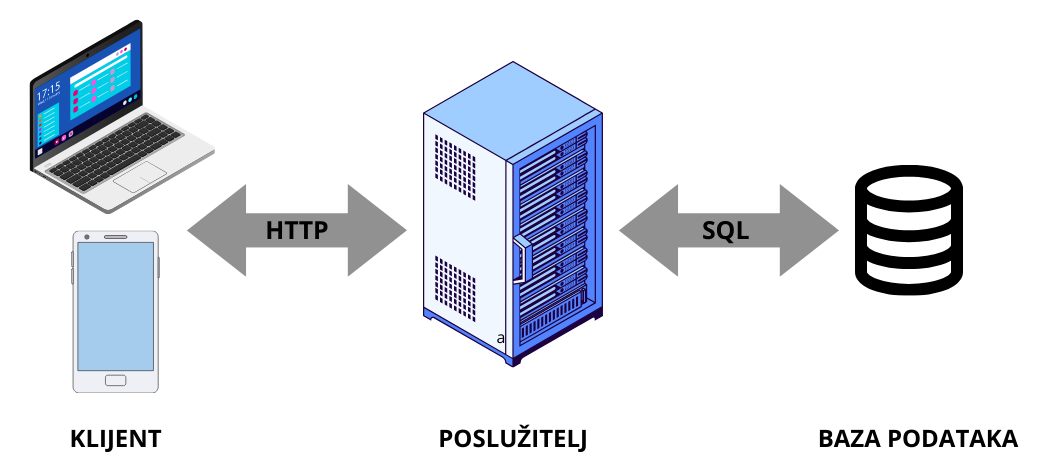
\includegraphics[scale=0.4]{slike/arh1.PNG} %veličina slike u odnosu na originalnu datoteku i pozicija slike
						\centering
						\caption{Organizacija sustava s najviše razine apstrakcije}
						\label{fig:promjene4}
					\end{figure}	
	Arhitektura aplikacije je troslojna. Prvi sloj je \textbf {kontroler} koji prima zahtjeve, poziva odgovarajuće metode drugog sloja \textbf {servisa}, te na kraju vraća odgovore. Servis sadrži poslovnu logiku aplikacije, a za pristup podacima koristi treći sloj \textbf {repozitorij} koji komunicira s bazom podataka.
					\begin{figure}[H]
						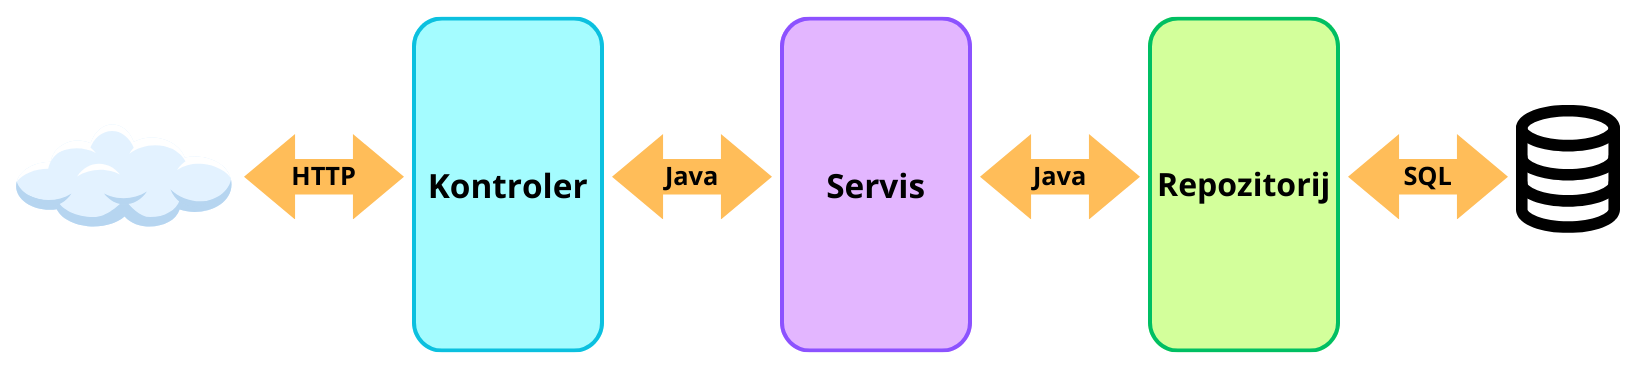
\includegraphics[scale=0.3]{slike/arh2.PNG} %veličina slike u odnosu na originalnu datoteku i pozicija slike
						\centering
						\caption{Organizacija aplikacije}
						\label{fig:promjene5}
					\end{figure}	
	Za izradu naše aplikacije korišten je Java Spring Boot okvir koji koristi MVC \textit{(engl. Model-View-Controller)} oblikovni obrazac u kojem je poslužitelj organiziran u tri dijela u cilju razdvajanja nadležnosti. Aplikacija je podijeljena na tri komponente. \textbf {Kontroler} prima zahtjeve koje prosljeđuje modelu te upravlja modelom i pogledom. \textbf {Model} je zadužen za obradu i dohvat podataka te komunicira s bazom podataka. \textbf {Pogled} prezentira dostavljene podatke.
	
		

		

				
		\section{Baza podataka}
		U aplikaciji će baza podataka bit prikazana relacijskim modelom podataka. Objekti relacijskog modela su relacije, a svaka ima jedinstveno ime unutar sheme baze podataka. Relacija je tablica čiji se imenovani stupci nazivaju atributi, a redci n-torke. Ključ entiteta je skup atributa koji jednoznačno određuje entitet. U našem sustavu entiteti baze podataka su:
	\begin{itemize}
		\item Rad
		\item Osoba
		\item Konferencija
		\item Prisutan\_na
		\item Mjesto
		\item Fotografija
		\item Pokrovitelj	
		\item Pokrovitelj\_na	
	\end{itemize}
			\subsection{Opis tablica}
			Entitet \textbf {Rad} sadrži sve važne informacije o radu. Sadrži atribute: ID rada, naziv postera, naziv prezentacije, naslov rada, ID autora, ID konferencije na koju je prijavljen i ukupan broj osvojenih glasova na toj konferenciji. Atribut naziv prezentacije je opcionalan te stoga može poprimiti vrijednost null. Entitet Rad u binarnoj je vezi s \textit{(Many-to-One)} s entitetom Konferencija i u vezi \textit{(Many-to-One)} s entitetom Osoba, odnosno onim njegovim n-torkama kojima je vrijednost atributa uloga "autor".
				\begin{longtblr}[
					label=none,
					entry=none
					]{
						width = \textwidth,
						colspec={|X[7,l]|X[6, l]|X[20, l]|}, 
						rowhead = 1,
					} %definicija širine tablice, širine stupaca, poravnanje i broja redaka naslova tablice
					\hline \SetCell[c=3]{c}{\textbf{Rad}}	 \\ \hline[3pt]
					\SetCell{LightGreen}id & SERIAL	&  	jedinstveni identifikator rada 	\\ \hline
					nazivPoster	& VARCHAR &   	naziv postera koji prikazuje rad\\ \hline 
					nazivPptx & VARCHAR &   naziv prezentacije koja prikazuje rad, može biti null\\ \hline 
					naslov & VARCHAR	&    naslov rada\\ \hline 
					ukupnoGlasova & INT &   ukupan broj osvojenih glasova na konferenciji\\ \hline 
					\SetCell{LightBlue}idKonf	& SERIAL &   	jedinstveni identifikator konferencije\\ \hline 
					\SetCell{LightBlue}idAutor & SERIAL&    jedinstveni identifikator autora\\ \hline 
				\end{longtblr}						
			
			\noindent Entitet \textbf {Osoba} sadrži informacije o autorima, korisnicima te adminima. Sadrži atribute: ID osobe, email, ime i prezime, lozinka (u slučaju da se radi o autoru koji ujedno nije i korisnik bit će null) i uloga koji može poprimiti vrijednost "admin", "korisnik" i "autor". Entitet Osoba (uloga autor) u binarnoj je vezi s entitetom Rad \textit{(One-to-Many)}, (uloga admin) s entitetom Konferencija \textit{(One-to-Many)}, (uloga korisnik) s entitetom Konferencija \textit{(Many-to-Many)}.
				\begin{longtblr}[
					label=none,
					entry=none
					]{
						width = \textwidth,
						colspec={|X[7,l]|X[6, l]|X[20, l]|}, 
						rowhead = 1,
					} %definicija širine tablice, širine stupaca, poravnanje i broja redaka naslova tablice
					\hline \SetCell[c=3]{c}{\textbf{Osoba}}	 \\ \hline[3pt]
					\SetCell{LightGreen}id & SERIAL	&  	jedinstveni identifikator osobe\\ \hline
					email	& VARCHAR &   	email osobe\\ \hline 
					ime & VARCHAR &   ime osobe\\ \hline 
					prezime & VARCHAR	&    prezime osobe\\ \hline 
					lozinka & VARCHAR &   hash lozinke korisnika ili admina\\ \hline 
					uloga & VARCHAR &  uloga osobe\\ \hline 
				\end{longtblr}		

			\noindent Entitet \textbf {Konferencija} sadrži informacije o stručnoj konferenciji koja će se održati. Sadrži atribute: ID konferencije, poveznica na video prijenos konferencije, pin za ulazak na konferenciju, vrijeme početka i vrijeme kraja konferencije, ID admina zaduženog za konferenciju i poštanski broj mjesta u kojem se održava konferencija. Entitet Konferencija u binarnoj je vezi s entitetom Rad \textit{(One-to-Many)}, u binarnoj vezi \textit{(Many-to-One)} s entitetom Osoba, odnosno s onim njegovim n-torkama kojima je vrijednost atributa uloga "admin" i \textit{(Many-to-Many)} s n-torkama kojima je vrijednost atributa uloga "korisnik", u vezi \textit{(Many-to-One)} s entitetom Mjesto, \textit{(One-to-Many)} s entitetom Fotografija i \textit{(Many-to-Many)} s entitetom Pokrovitelj.
				\begin{longtblr}[
					label=none,
					entry=none
					]{
						width = \textwidth,
						colspec={|X[6,l]|X[6, l]|X[20, l]|}, 
						rowhead = 1,
					} %definicija širine tablice, širine stupaca, poravnanje i broja redaka naslova tablice
					\hline \SetCell[c=3]{c}{\textbf{Konferencija}}	 \\ \hline[3pt]
					\SetCell{LightGreen}id & SERIAL	&  	jedinstveni identifikator konferencije \\ \hline
					urlVideo	& VARCHAR &   	 poveznica na direktno video praćenje
trenutnih događanja u glavnoj konferencijskoj dvorani\\ \hline 
					pin & INT &   jedinstveni pin konferencije\\ \hline 
					vrijemePocetak & TIMESTAMP	&    početak konferencije\\ \hline 
					vrijemeKraj & TIMESTAMP	&    kraj konferencije\\ \hline 
					\SetCell{LightBlue} idAdmin & SERIAL &   jedinstveni identifikator admina zaduženog za konferenciju\\ \hline 
					\SetCell{LightBlue} pbr & INT &   poštanski broj mjesta u kojem se održava konferencija\\ \hline 
				\end{longtblr}		

			\noindent Entitet \textbf {Prisutan\_na} sadrži informacije o prisutnosti pojedinog korisnika na određenoj konferenciji te je li glasao na njoj ili ne. Sadrži atribute: ID konferencije, ID korisnika i glasao. Entitet Prisutan\_na rezultat je binarne veze \textit{(Many-to-Many)} entiteta Osoba, odnosno veze onih njegovih n-torka kojima je vrijednost atributa uloga "korisnik" s entitetom Konferencija.
				\begin{longtblr}[
					label=none,
					entry=none
					]{
						width = \textwidth,
						colspec={|X[6,l]|X[6, l]|X[20, l]|}, 
						rowhead = 1,
					} %definicija širine tablice, širine stupaca, poravnanje i broja redaka naslova tablice
					\hline \SetCell[c=3]{c}{\textbf{Prisutan\_na}}	 \\ \hline[3pt]
					\SetCell{LightGreen}idKonf & SERIAL	&  	jedinstveni identifikator konferencije \\ \hline
					\SetCell{LightGreen}idKorisnik	& SERIAL &   	jedinstveni identifikator korisnika\\ \hline 
					glasao & BOOLEAN &   informacija je li korisnik već glasao na konferenciji\\ \hline 
				\end{longtblr}

			\noindent Entitet \textbf {Mjesto} sadrži informacije o pojedinom mjestu. Sadrži atribute: poštanski broj i naziv mjesta. Entitet Mjesto u binarnoj je vezi s entitetom Konferencija \textit{(One-to-Many)}. 
				\begin{longtblr}[
					label=none,
					entry=none
					]{
						width = \textwidth,
						colspec={|X[6,l]|X[6, l]|X[20, l]|}, 
						rowhead = 1,
					} %definicija širine tablice, širine stupaca, poravnanje i broja redaka naslova tablice
					\hline \SetCell[c=3]{c}{\textbf{Mjesto}}	 \\ \hline[3pt]
					\SetCell{LightGreen}pbr & INT &   poštanski broj mjesta \\ \hline
					naziv	& VARCHAR &   	naziv mjesta\\ \hline 
				\end{longtblr}

			\noindent Entitet \textbf {Fotografija} sadrži informacije o uslikanoj fotografiji te na kojoj konferenciji je uslikana. Sadrži atribute: ID fotografije, naziv fotografije i ID konferencije. Entitet Fotografija u binarnoj je vezi s entitetom Konferencija \textit{(Many-to-One)}. 
				\begin{longtblr}[
					label=none,
					entry=none
					]{
						width = \textwidth,
						colspec={|X[6,l]|X[6, l]|X[20, l]|}, 
						rowhead = 1,
					} %definicija širine tablice, širine stupaca, poravnanje i broja redaka naslova tablice
					\hline \SetCell[c=3]{c}{\textbf{Fotografija}}	 \\ \hline[3pt]
					\SetCell{LightGreen}id & SERIAL	&  	jedinstveni identifikator fotografije\\ \hline
					naziv	& VARCHAR &   	naziv fotografije\\ \hline 
					\SetCell{LightBlue}idKonf & SERIAL &   jedinstveni identifikator konferencije\\ \hline 
				\end{longtblr}

			\noindent Entitet \textbf {Pokrovitelj} sadrži informacije o pokrovitelju. Sadrži atribute: ID pokrovitelja,  url stranice pokrovitelja i naziv pokrovitelja. Entitet Pokrovitelj u binarnoj je vezi s entitetom Konferencija \textit{(Many-to-Many)}. 
				\begin{longtblr}[
					label=none,
					entry=none
					]{
						width = \textwidth,
						colspec={|X[7,l]|X[6, l]|X[20, l]|}, 
						rowhead = 1,
					} %definicija širine tablice, širine stupaca, poravnanje i broja redaka naslova tablice
					\hline \SetCell[c=3]{c}{\textbf{Pokrovitelj}}	 \\ \hline[3pt]
					\SetCell{LightGreen}id & SERIAL	&  	jedinstveni identifikator pokrovitelja\\ \hline
					url	& VARCHAR &   	poveznica na stranicu pokrovitelja\\ \hline 
					naziv	& VARCHAR &   	naziv pokrovitelja\\ \hline 
				\end{longtblr}

			\noindent Entitet \textbf {Pokrovitelj\_na} sadrži informacije o uključenosti pokrovitelja na pojedinoj konferenciji. Sadrži atribute: ID konferencije i ID pokrovitelja. Entitet Pokrovitelj\_na rezultat je binarne veze \textit{(Many-to-Many)} entiteta Pokrovitelj i Konferencija.
				\begin{longtblr}[
					label=none,
					entry=none
					]{
						width = \textwidth,
						colspec={|X[6,l]|X[6, l]|X[20, l]|}, 
						rowhead = 1,
					} %definicija širine tablice, širine stupaca, poravnanje i broja redaka naslova tablice
					\hline \SetCell[c=3]{c}{\textbf{Pokrovitelj\_na}}	 \\ \hline[3pt]
					\SetCell{LightGreen}idKonf & SERIAL	&  	jedinstveni identifikator konferencije \\ \hline
					\SetCell{LightGreen}idPokrovitelj	& SERIAL &   	jedinstveni identifikator pokrovitelja\\ \hline 
				\end{longtblr}
	
			\subsection{Dijagram baze podataka}
%				\textit{ U ovom potpoglavlju potrebno je umetnuti dijagram baze podataka. Primarni i strani ključevi moraju biti označeni, a tablice povezane. Bazu podataka je potrebno normalizirati. Podsjetite se kolegija "Baze podataka".}
					\begin{figure}[H]
						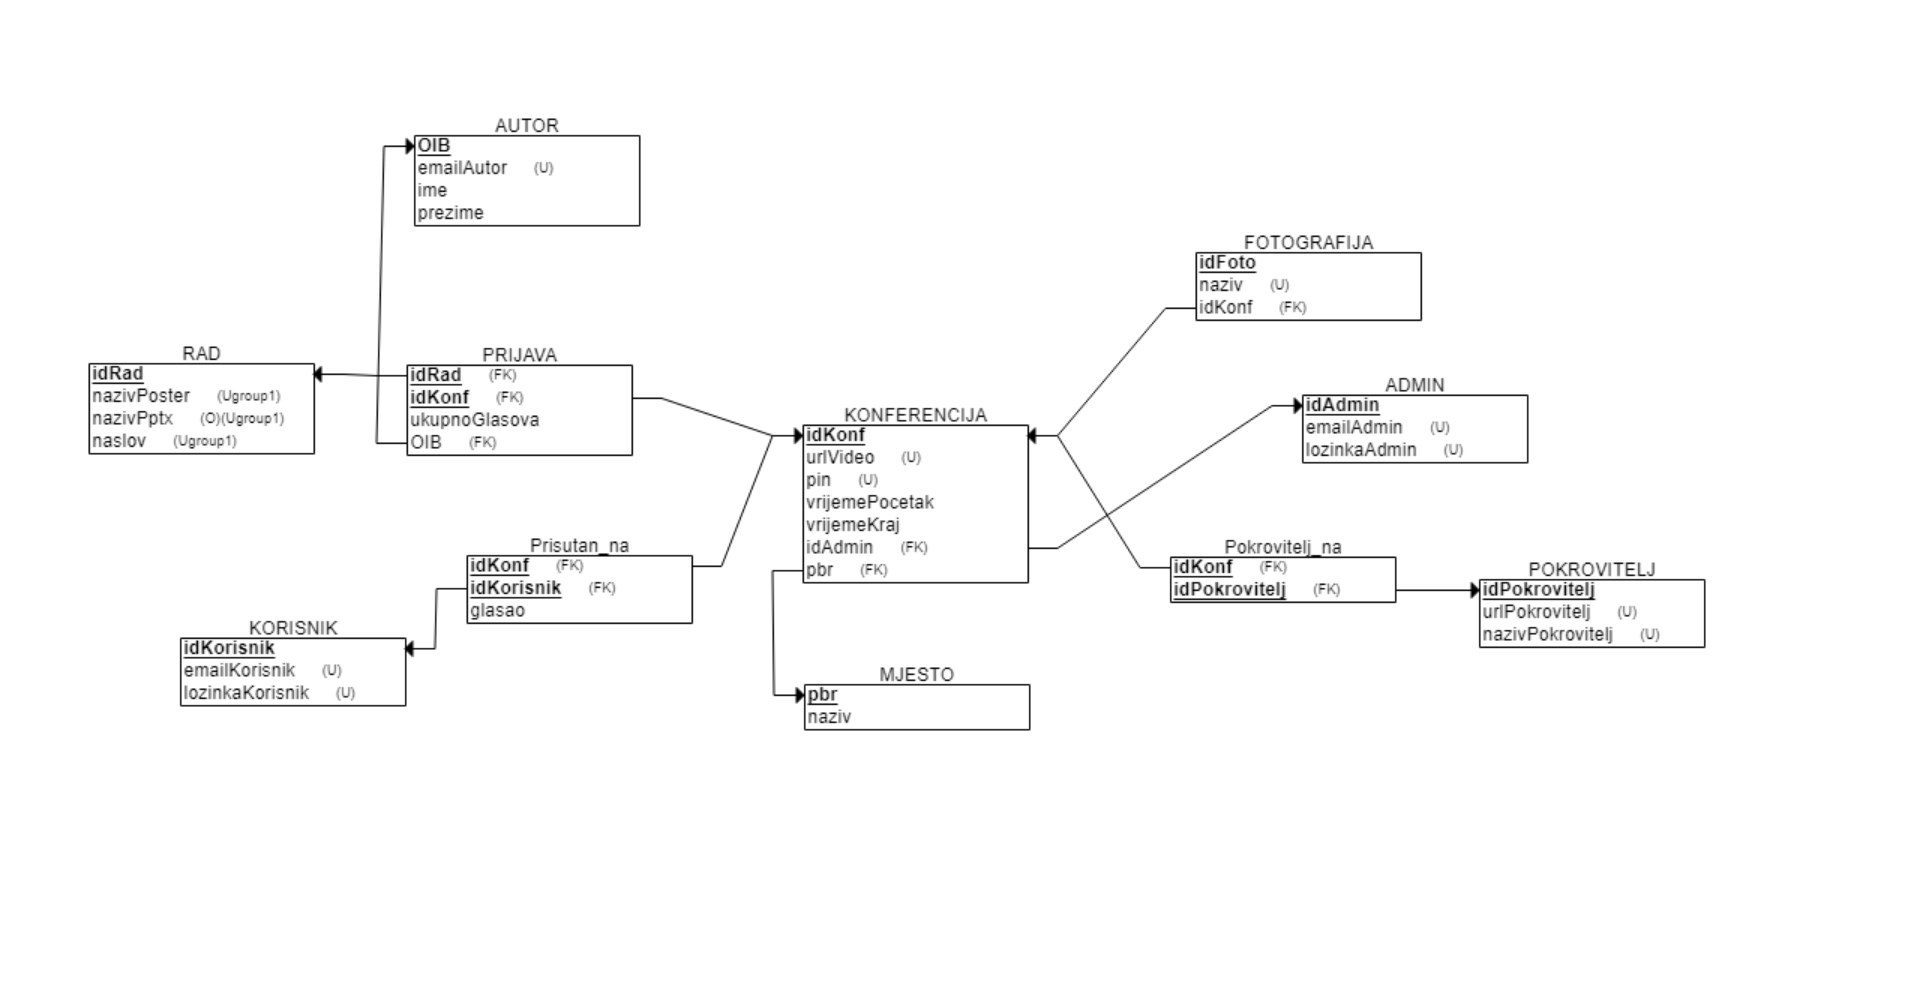
\includegraphics[scale=0.55]{slike/dijagram baze podataka.PNG} %veličina slike u odnosu na originalnu datoteku i pozicija slike
						\centering
						\caption{Dijagram baze podataka}
						\label{fig:promjene3}
					\end{figure}			
			\eject
			
			
		\section{Dijagram razreda}
		
		
			Radi preglednosti, dijagram je razlomljen na nekoliko dijelova. Na njima su prikazani razredi koji pripadaju backend dijelu MVC arhitekture.
			Na slici 4.4 su prikazane DTO klase. DTO klase služe za prijenos podataka između baze podataka i serverske strane aplikacije. Ti su objekti zapravo preslika baze podataka, ali umjesto relacijske koristimo objektno-orijentiranu paradigmu. 
			Razred Konferencija predstavlja konferenciju koja se prikazuje u aplikaciji. 
Razred Mjesto predstavlja lokaciju na kojoj se konferencija održava.
Razred Osoba predstavlja čovjeka koji na neki način sudjeluje na konferenciji.  Taj razred ima atribut uloga kojim se određuje je li ta osoba autor, administrator ili posjetitelj konferencije. 
Razred Rad predstavlja rad (poster i/ili pptx) kojim se autor predstavlja na konferenciji.
Razred PrisutanNa omogućuje da pratimo tko je na konferenciji te da li je ta osoba glasala za neki rad.
Razred Fotografija predstavlja fotografije konferencije koje administrator stavlja u aplikaciju tijekom ili nakon konferencije.
Razred Pokrovitelj predstavlja sponzore konferencije. 

			\begin{figure}[H]
				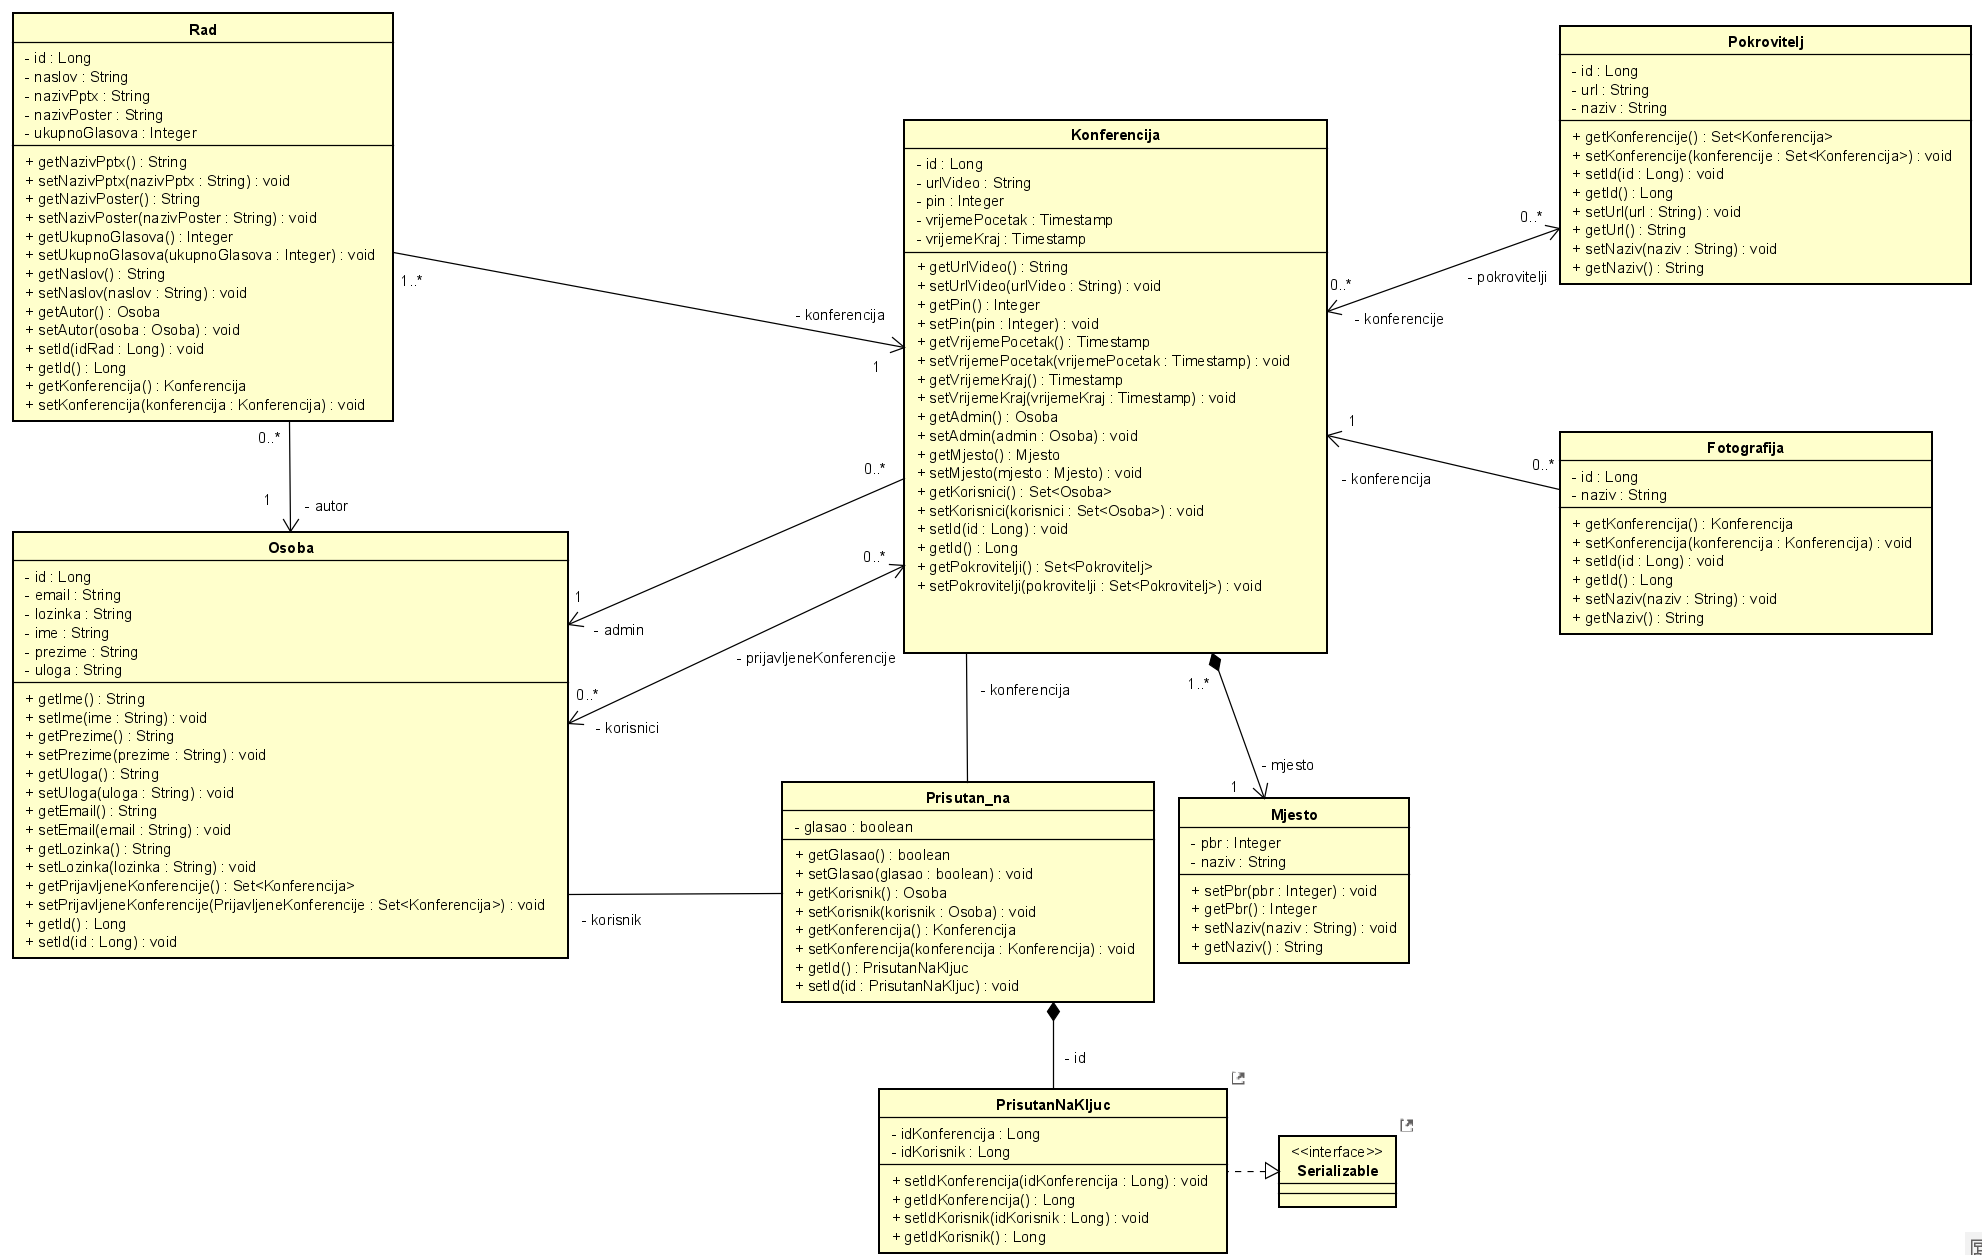
\includegraphics[scale=0.4]{slike/dto_klase.png}%veličina slike u odnosu na originalnu datoteku i pozicija slike
				\centering
				\caption{Dijagram razreda - DTO}
				\label{fig:promjena9}
			\end{figure}
			

			Na slikama 4.5, 4.6, 4.7 je prikazan glavni dijagram u čijem središtu se nalazi JPARepository o kojem ovise ostala sučelja koja su specifična za svaki objekt. Ova sučelja nam omogućuju da izbjegnemo pisanje složenih SQL upita i umjesto toga koristimo generičke metode za izvođenje uobičajenih operacija s bazom podataka.
U dijagramu su i servisi u kojima su funkcije za obradu podataka. Po potrebi zovu repozitorijeve funkcije kako bi došli do baze podataka.
Kontroleri nam služe za komunikaciju s frontendom. 
U klasi PosterizedApplication se nalazi glavna funkcija za pokretanje aplikacije. WebSecurityBasic je zadužen za zaštitu cijele aplikacije.

			

			\begin{figure}[H]
				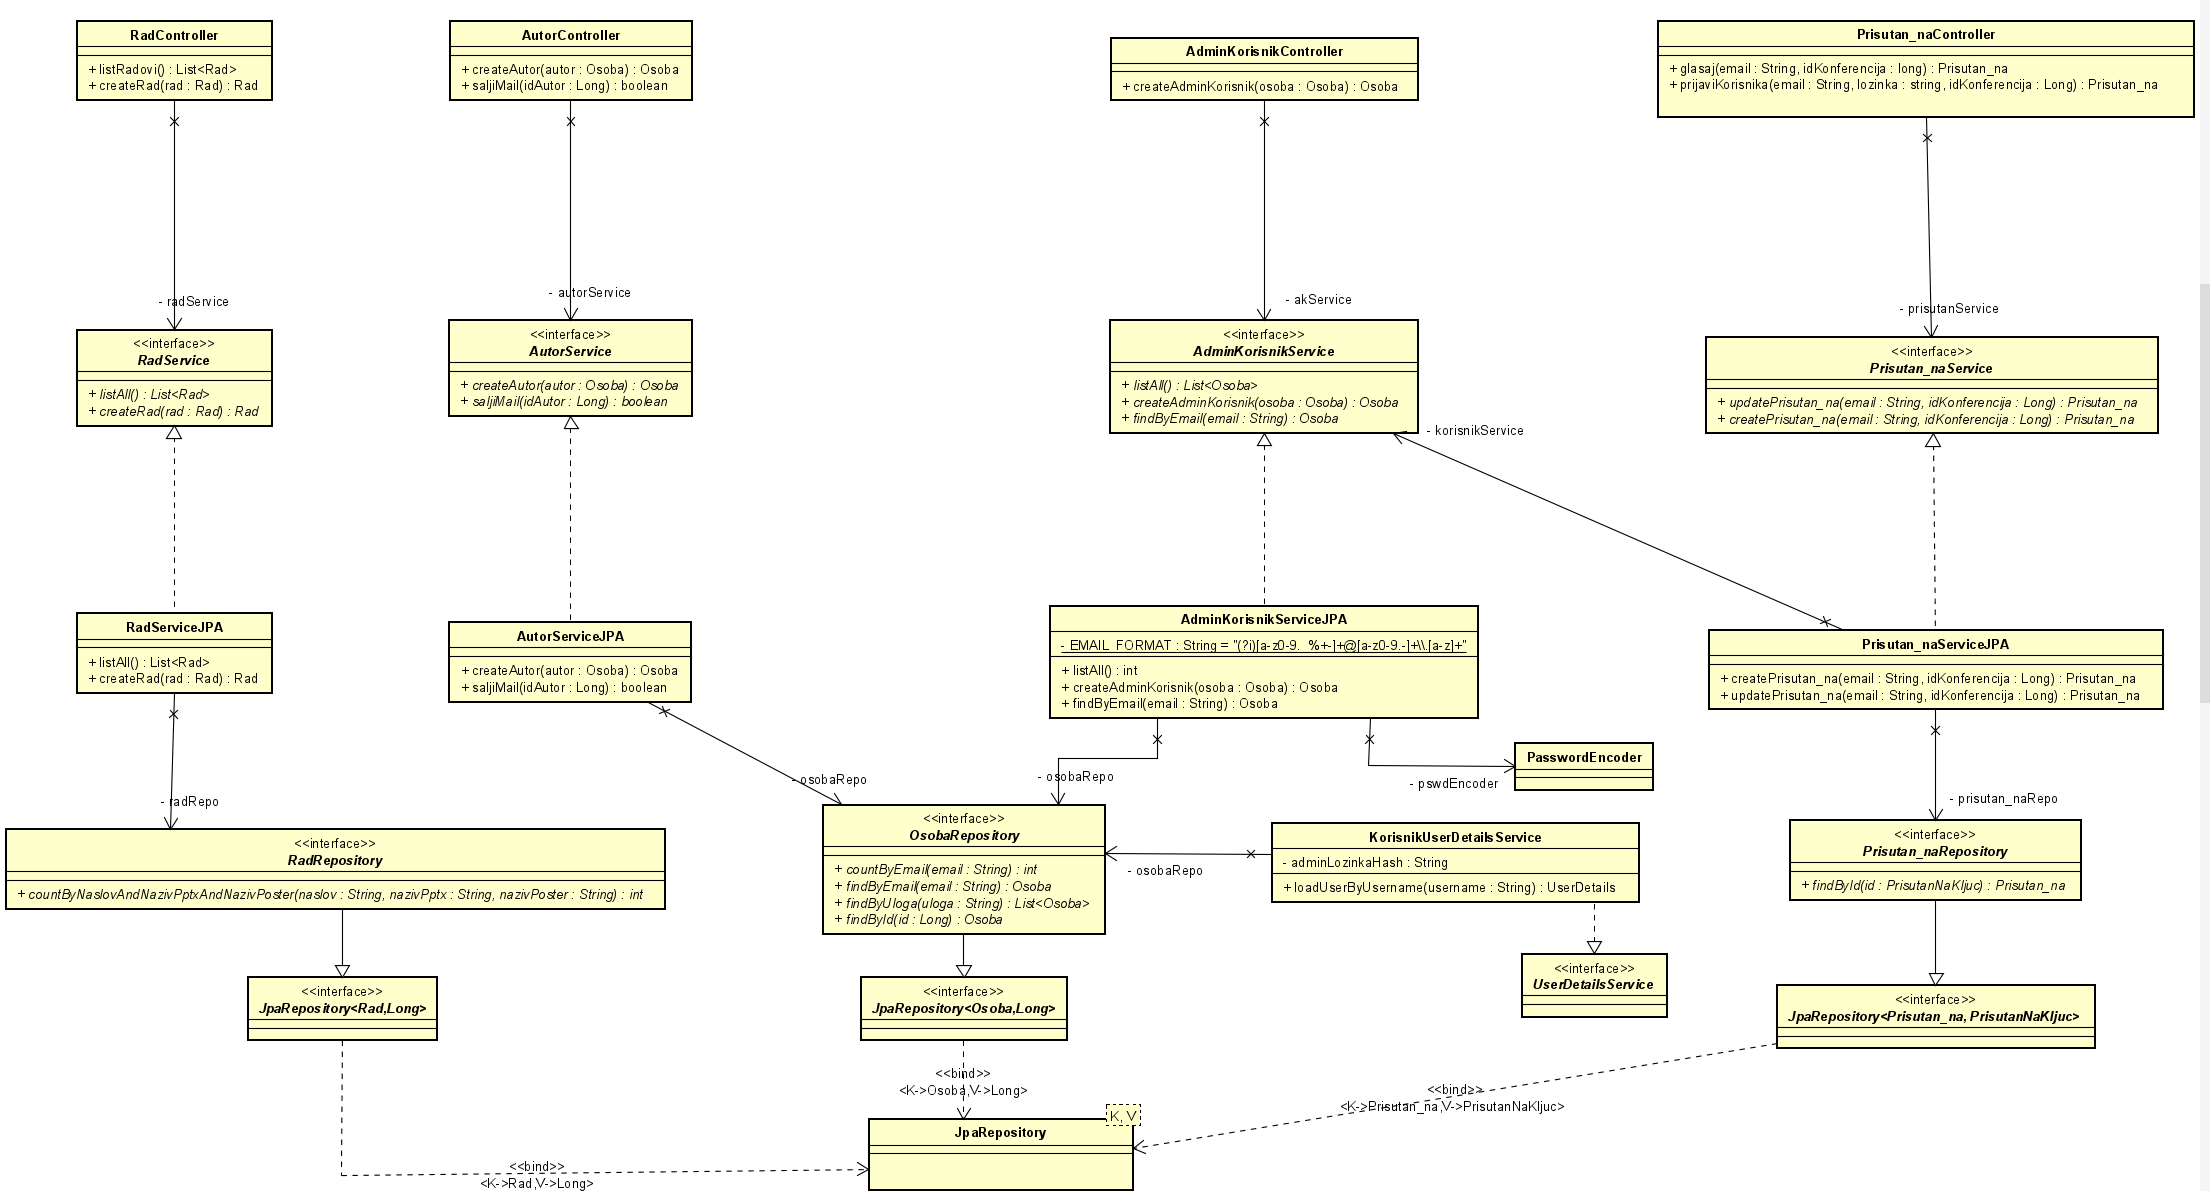
\includegraphics[scale=0.4]{slike/glavni_1.png}%veličina slike u odnosu na originalnu datoteku i pozicija slike
				\centering
				\caption{Dijagram razreda - glavni dijagram 1.dio}
				\label{fig:promjena9.1}
			\end{figure}
			
			\begin{figure}[H]
				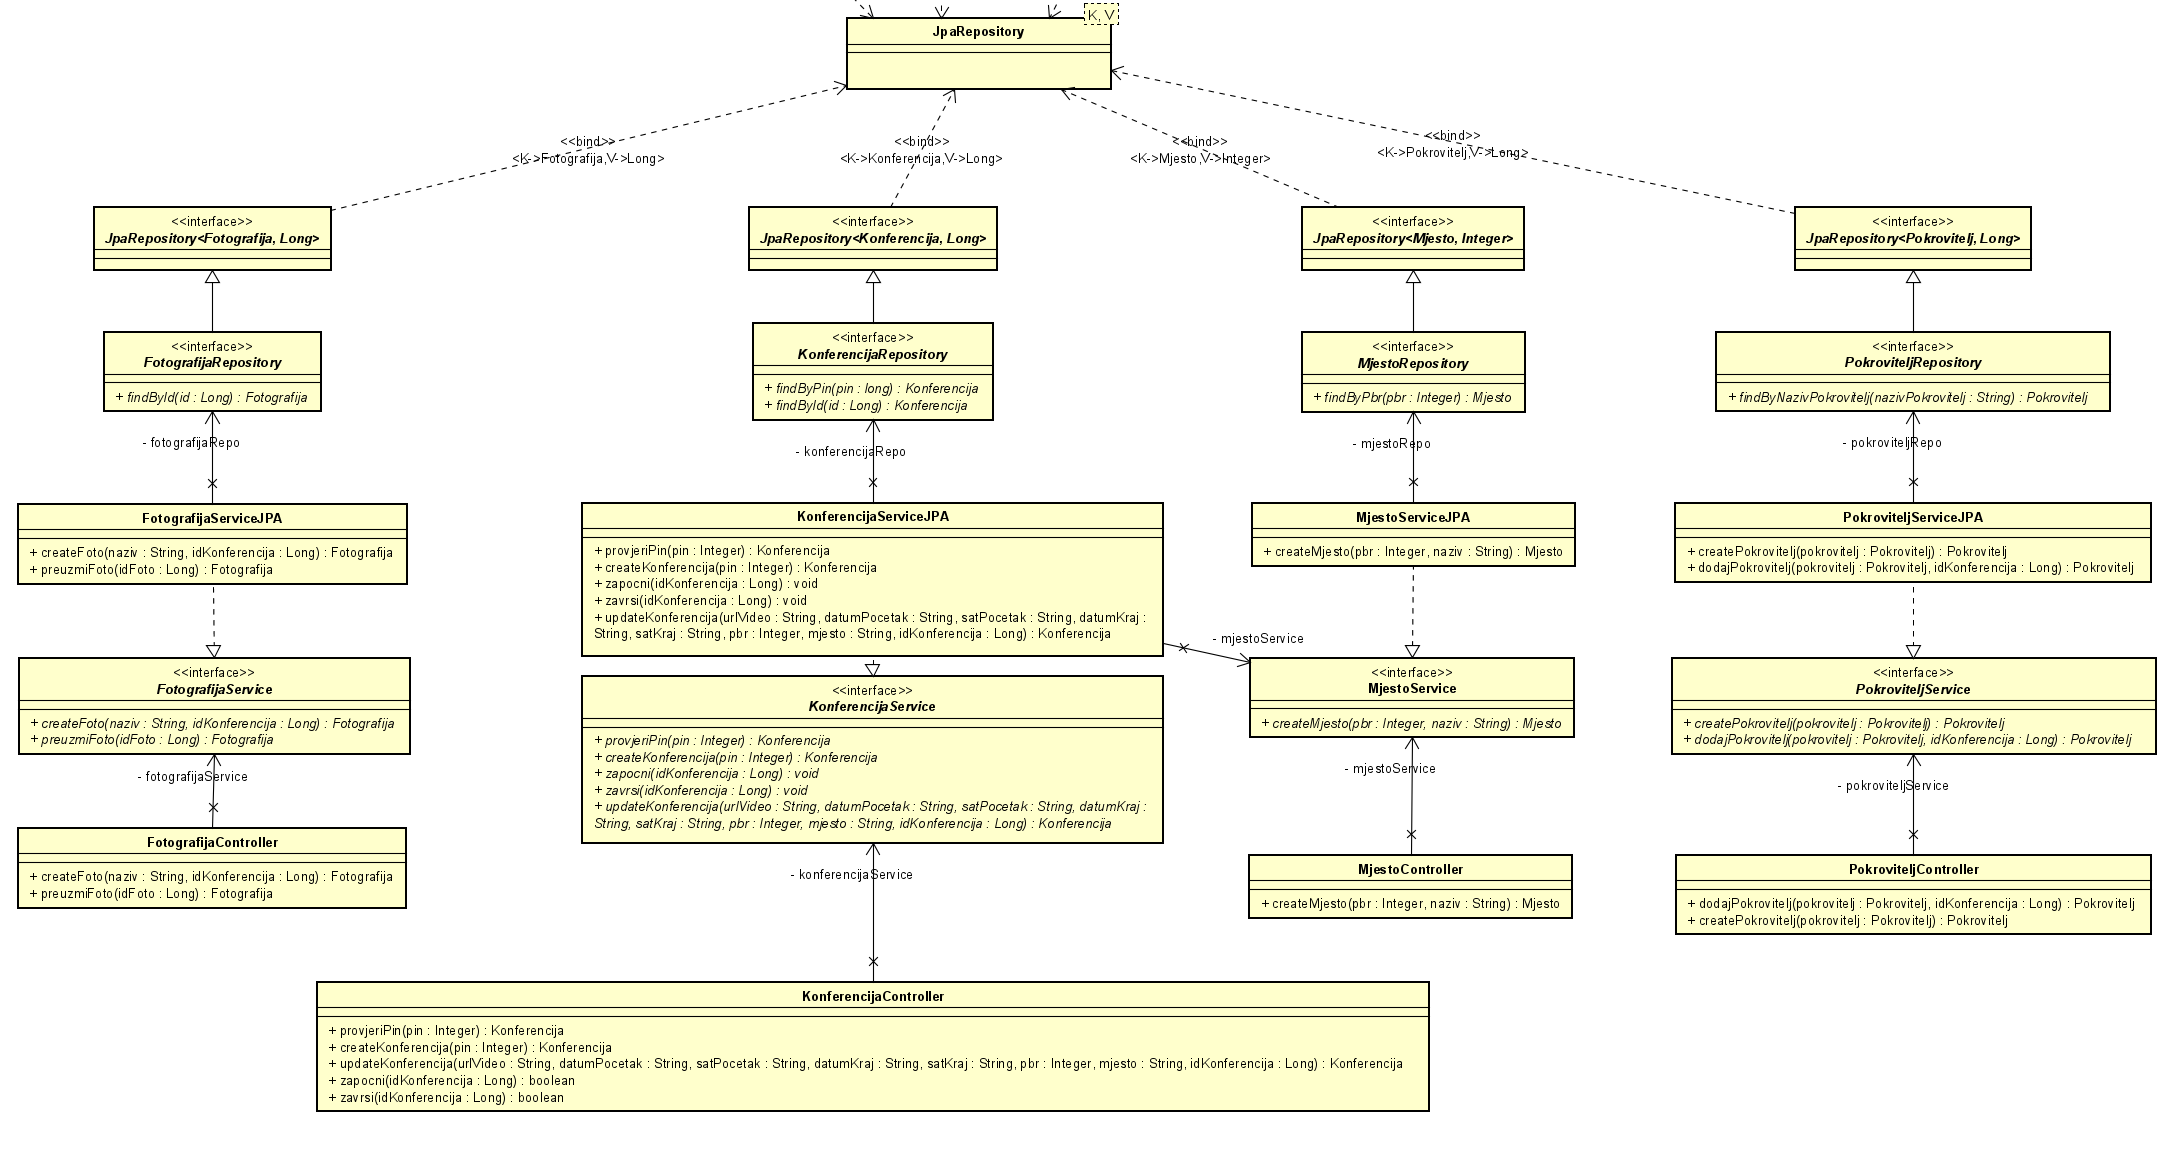
\includegraphics[scale=0.4]{slike/glavni_2.png}%veličina slike u odnosu na originalnu datoteku i pozicija slike
				\centering
				\caption{Dijagram razreda - glavni dijagram 2.dio}
				\label{fig:promjena9.2}
			\end{figure}
			
			\begin{figure}[H]
				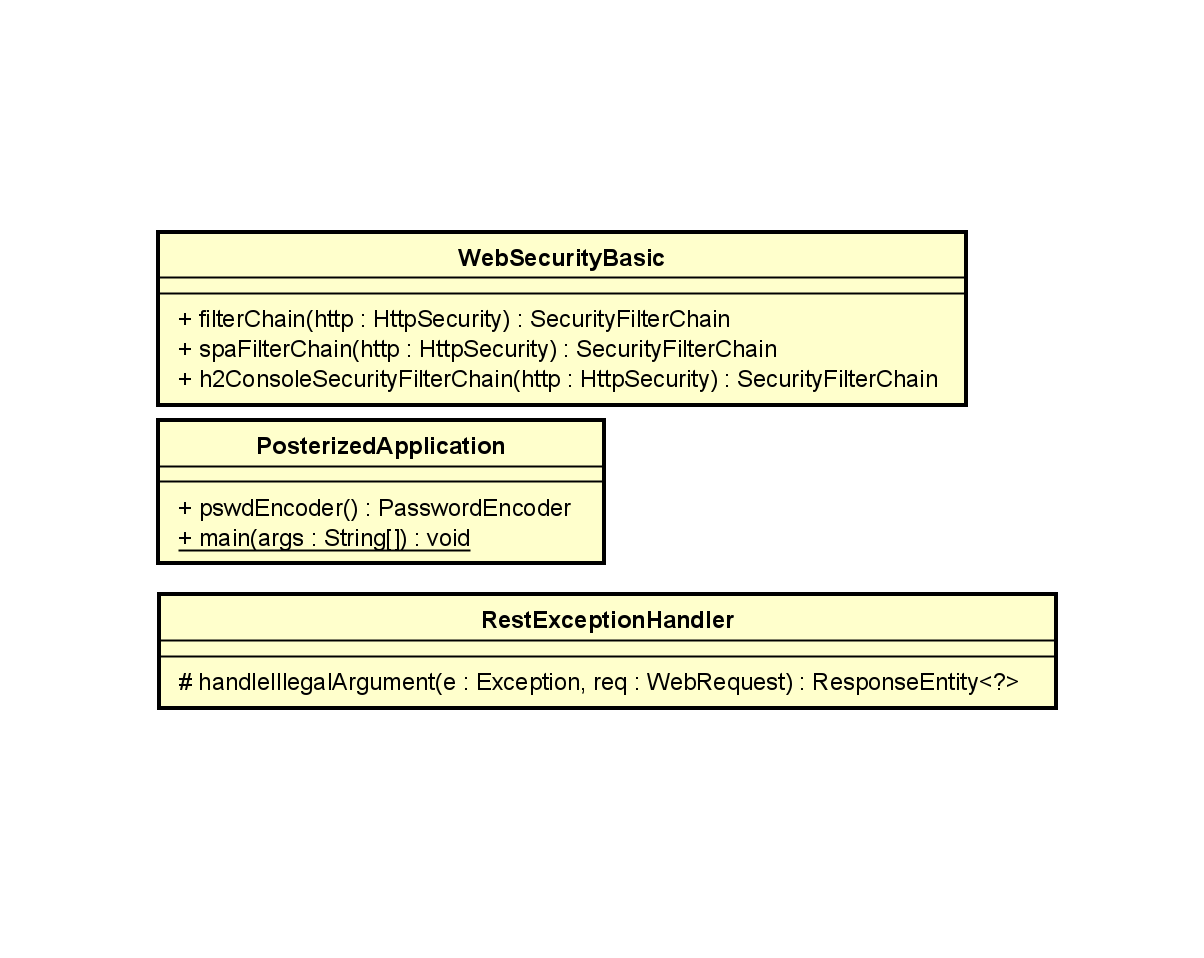
\includegraphics[scale=0.5]{slike/glavni_3.png}%veličina slike u odnosu na originalnu datoteku i pozicija slike
				\centering
				\caption{Dijagram razreda - glavni dijagram 3.dio}
				\label{fig:promjena9.3}
			\end{figure}
			\eject



			\textbf{\textit{dio 2. revizije}}\\			
			
			\textit{Prilikom druge predaje projekta dijagram razreda i opisi moraju odgovarati stvarnom stanju implementacije}
			
			
			
			\eject
		
		\section{Dijagram stanja}
			
			
			\textbf{\textit{dio 2. revizije}}\\
			
			\textit{Potrebno je priložiti dijagram stanja i opisati ga. Dovoljan je jedan dijagram stanja koji prikazuje \textbf{značajan dio funkcionalnosti} sustava. Na primjer, stanja korisničkog sučelja i tijek korištenja neke ključne funkcionalnosti jesu značajan dio sustava, a registracija i prijava nisu. }
			
			
			\eject 
		
		\section{Dijagram aktivnosti}
			
			\textbf{\textit{dio 2. revizije}}\\
			
			 \textit{Potrebno je priložiti dijagram aktivnosti s pripadajućim opisom. Dijagram aktivnosti treba prikazivati značajan dio sustava.}
			
			\eject
		\section{Dijagram komponenti}
		
			\textbf{\textit{dio 2. revizije}}\\
		
			 \textit{Potrebno je priložiti dijagram komponenti s pripadajućim opisom. Dijagram komponenti treba prikazivati strukturu cijele aplikacije.}